% CVPR 2023 Paper Template
% based on the CVPR template provided by Ming-Ming Cheng (https://github.com/MCG-NKU/CVPR_Template)
% modified and extended by Stefan Roth (stefan.roth@NOSPAMtu-darmstadt.de)

\documentclass[10pt,twocolumn,letterpaper]{article}

%%%%%%%%% PAPER TYPE  - PLEASE UPDATE FOR FINAL VERSION
\usepackage{cvpr}      % To produce the REVIEW version


% Include other packages here, before hyperref.
\usepackage{graphicx}
\usepackage{amsmath}
\usepackage{amssymb}
\usepackage{booktabs}
\usepackage{enumitem}
\usepackage{csquotes}

% It is strongly recommended to use hyperref, especially for the review version.
% hyperref with option pagebackref eases the reviewers' job.
% Please disable hyperref *only* if you encounter grave issues, e.g. with the
% file validation for the camera-ready version.
%
% If you comment hyperref and then uncomment it, you should delete
% ReviewTempalte.aux before re-running LaTeX.
% (Or just hit 'q' on the first LaTeX run, let it finish, and you
%  should be clear).
\usepackage[pagebackref,breaklinks,colorlinks]{hyperref}


% Support for easy cross-referencing
\usepackage[capitalize]{cleveref}
\crefname{section}{Sec.}{Secs.}
\Crefname{section}{Section}{Sections}
\Crefname{table}{Table}{Tables}
\crefname{table}{Tab.}{Tabs.}


%%%%%%%%% PAPER ID  - PLEASE UPDATE
\def\cvprPaperID{*****} % *** Enter the CVPR Paper ID here
\def\confName{CVPR}
\def\confYear{2023}


\begin{document}

%%%%%%%%% TITLE - PLEASE UPDATE
\title{Team \#16: From Strings to Sequences --- Classifying and Generating Music from Acoustic Guitar Notes}

\author{
    Camilo Martínez\\
    7057573\\
    \and
    Dhimitrios Duka\\
    7059153\\
    \and
    Honglu Ma\\
    7055053\\
}
\maketitle

%%%%%%%%% BODY TEXT
\section{Task and Motivation}
Automatic cord recognition (ACR) consists of recognizing the chords played in a music piece. This information is quite valuable since it can later be used for music analysis, music transcription, or even fixing corrupted musical performances. ACR was first introduced in 1999 by \cite{takuya1999realtime} where the author utilized lisp music to perform chord recognition at the signal level. Since then, many signal-level-based approaches have been introduced. However, these methods proved to be quite challenging and not very accurate.

With the rise of deep learning, and especially computer vision, many researchers started to tackle this problem from a different perspective. They began to use spectrogram-based feature extraction methods to extract the features of the audio signal \cite{boulanger2013audio, korzeniowski2016feature, stark2009real}. However, despite the success of these methods, improvements plated \blockquote{due to the inherent shortcomings of the aural approach in handling highly timbre sounds} \cite{du2023conditional}.

Inspired by the fact that for most people it is easier to distinguish a note from a visual aspect rather than the sound of it, researchers started to come up with methods that leverage this fact. \cite{su2020audeo} successfully reconstructed audio from a video of a piano being played. However, the technique was only applied to a digital render of a piano, which does not depict a real-world scenario as no human was interacting with it.

Building on the concept of using visual information for musical applications, Y. Kristian et al. \cite{Kristian_Zaman_Tenoyo_Jodhinata_2024} employed a Single Shot Detection (SSD) model undergirded by a MobileNetV2 base model, pre-trained on the EgoHands dataset to achieve fretboard detection and chords classification. Their model generates coordinates for bounding boxes that outline the fretboard which in turn is used as the input for the chord classification model.

Our work builds on top of the previously mentioned works \cite{Kristian_Zaman_Tenoyo_Jodhinata_2024}
\cite{du2023conditional} and aims to improve the accuracy the chord recognition as well as implement a chord-to-audio generation model.

\section{Goals}

\begin{figure*}[h]
    \centering
    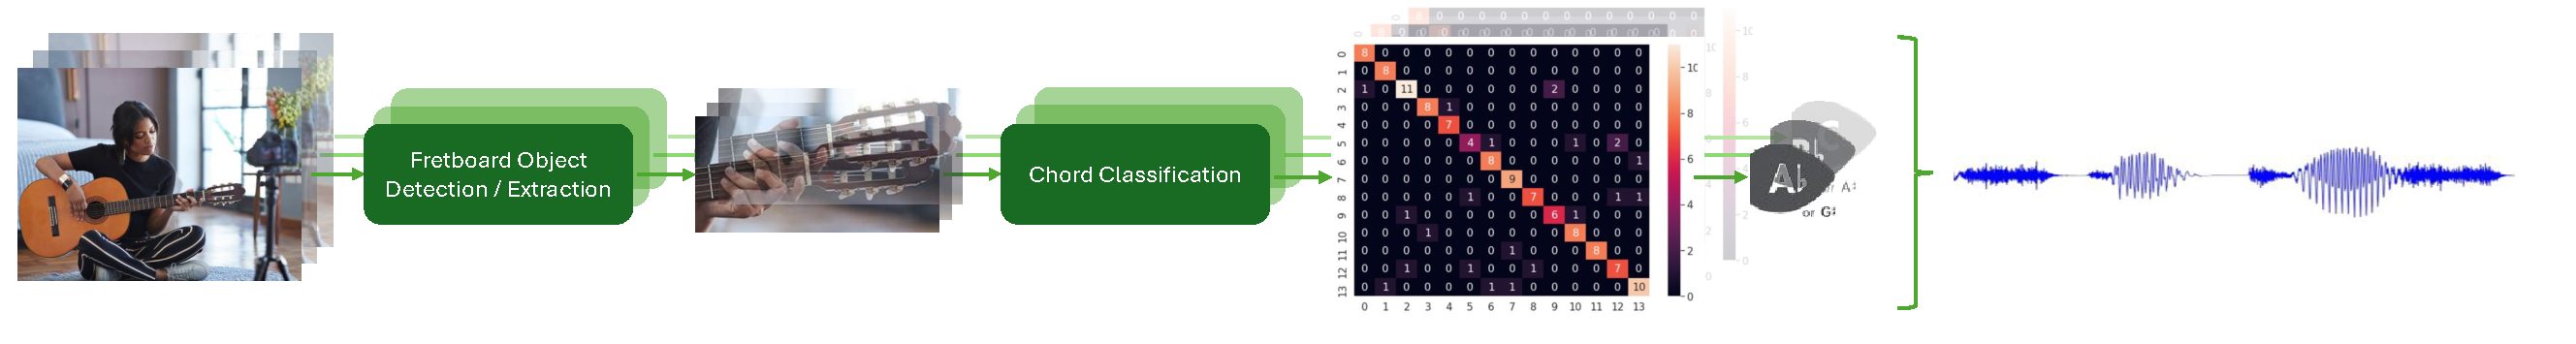
\includegraphics[width=\textwidth]{images/task-diagram.pdf}
    \caption{Overview of the Model, showcasing the 2 most important tasks:
        Fretboard Detection and Chord Classification, done for each frame of an input video. Image taken from \textit{Getty Stock Images}, confusion matrix image taken from \cite{Kristian_Zaman_Tenoyo_Jodhinata_2024}.}
    \label{fig:model-diagram}
\end{figure*}

\cref{fig:model-diagram} illustrates a bird's eye view of our model architecture. Essentially, we aim to address the following three problems:
\begin{enumerate}[label=\arabic*), itemsep=0.25pt]
    \item \emph{Fretboard Detection}: Given an image or video frame, detect the bounding box that outlines the fretboard.
    \item \emph{Chord Classification}: Given an image or video frame, classify the chord being played.
    \item \emph{Seamless Audio Generation}: Given the chords being played, generate the audio of the music piece.
\end{enumerate}
Y. Kristian et al. \cite{Kristian_Zaman_Tenoyo_Jodhinata_2024} focused on the first two problems, while we aim to address the third problem as well. This is a challenging task since it requires the model to seamlessly generate audio from the classified chords, effectively crossing into the \emph{generative} side of Neural Networks. That is, we aim to move beyong chord classification to also include audio synthesis. In Section \cref{sec:methods} and \cref{sec:datasets}, we briefly cover the methods and datasets we plan to use to address these challenges.

By the mid-term, we aim to have completed data collection and pruning, the code for pre-training a YOLO architecture for the \emph{fretboard detection model}, and the \emph{guitar chords classifier model}. By the end of the project, we aim to have the \emph{seamless audio generation model} completed.

\section{Methods}\label{sec:methods}

What models/frameworks do you use to solve the challenges?
We are expecting to use the following models to solve the challenges:
\begin{enumerate}[label=\arabic*), itemsep=0.25pt]
    \item \textbf{Fretboard Detection}: We plan to use YOLOv9 \cite{wang2024yolov9} and fine-tune it for fretboard detection using the datasets metioned in \cref{sec:datasets}.
    \item \textbf{Chord Classification}: We plan to use a tranformer based approach, mainly ViT \cite{dosovitskiy2020image}, and fine-tune it for guitar chord classification using the datasets metioned in \cref{sec:datasets}.
    \item \textbf{Seamless Audio Generation}: We plan to try both a plain decoder architecture and a transformer based approach, MelodyDiffusion \cite{math11081915}.
\end{enumerate}

But, if deemed necessary, we will also explore other models.

Why can the proposed method / analysis solve your problem?

As we're using state-of-the-art models, we expect to achieve better results than the previous work. Furthermore, by including the \emph{seamless audio generation model}, we aim to provide a more complete solution to the problem of automatic chord recognition.
Since the original video frames may be of different view points, orientations or environments, preprocessing the image with a fretboard detection model will help to standardize the input for the chord classification model.Though the visual transformer model has been shown to have ability to capture feature with a relatively small patch size, in our case, the fretboard cropping step will help us to focus on the finger positions with more details and reduce computational cost as well.

What are the main differences between your method and existing methods (if applicable)?
Unlike Y. Kristian et al. \cite{Kristian_Zaman_Tenoyo_Jodhinata_2024}, we do not plan to use Convolutional Neural Networks (CNNs) as a backbone for our approach. They used MobileNetV2 and MobileNetV1, which are CNN-based, for the fretboard detection and a Deep CNN for the chord classification.
Previous work 

What is the required computational budget for the training/analysis? (E.g. are you planning on using pretrained backbones?)

We are planning to use mostly pre-trained models and leverage transfer learning techniques. For the Seamless Audio Generation model we're expecting a higher computational budget, as most likely we will have to train the model from scratch.

\section{Datasets}\label{sec:datasets}

We have chosen the following datasets to train and evaluate our models, depending on the specific task to address: \emph{fretboard detection}, \emph{chord classification}, and \emph{seamless audio generation}. Furthermore, we follow the contributions of \cite{Kristian_Zaman_Tenoyo_Jodhinata_2024} and \cite{Jadhav_transferlearning} by first using three different pre-trained datasets to start off our models and leverage transfer learning techniques to improve the overall performance.
\subsection{Pre-trained Datasets}
The chosen datasets have each their own features, thus each one is used to pre-train a specific model.

\begin{enumerate}[label=\arabic*), itemsep=0.25pt]
    \item \textbf{ImageNet Dataset}: This dataset is used for pre-training our \emph{guitar chords classifier model}. It has over 14 million images that cover 20,000 types of natural objects \cite{russakovsky2015imagenetlargescalevisual}.
    \item \textbf{COCO Dataset}: This dataset is used for pre-training our \emph{fretboard detection model}. The dataset is of considerable size and is dedicated to object identification. Approximately 200,000 labeled images are organized into 80 distinct categories \cite{lin2015microsoftcococommonobjects}. Although somewhat comparable to ImageNet, the COCO dataset possesses a distinct emphasis.
    \item \textbf{EgoHands Dataset}: Similar to ImageNet, this dataset is also used for pre-training our \emph{guitar chords classifier model}. The dataset includes over 15,000 hand images with high-quality labels \cite{Bambach_2015_ICCV}.
    \item \textbf{GuitarSet}: This dataset is used for pre-training our \emph{seamless audio generation model} from the classified guitar chords. It provides high quality acoustic guitar recordings alongside time-aligned annotations including fret positions, chords, among others \cite{Xi2018}.
\end{enumerate}

\subsection{Fretboard Detection}\label{subsec:fretboard-detection}
To fine-tune the previously pre-trained \emph{fretboard detection model}, we will use the following datasets publicly available in \href{https://universe.roboflow.com/}{Roboflow}: \cite{guitar-chords-daewp_dataset}, \cite{guitar-ppfil_dataset} and \cite{done-npcll_dataset}.

\subsection{Chord Recognition}
To fine-tune the \emph{guitar chords classifier model}, we will use \cite{guitar-chord-tvon8_dataset}, \cite{guitar-chord-bounding-box_dataset}, \cite{guitar-chord-handshape_dataset}. Since \cite{guitar-chords-daewp_dataset} contains both the fretboard and the chords, we will use it to fine-tune this model as well.

\subsection{Seamless Audio Generation}
To fine-tune the \emph{seamless audio generation model}, we will use the \cite{Xi2018}.

\section{Evaluation}

Given the nature of our tasks (object detection, classification and audio generation), we do not need to define our own metric for evaluation. Instead, we will use the following metrics to evaluate the performance of our models.

\begin{enumerate}[label=\arabic*), itemsep=0.25pt]
    \item For the \emph{fretboard detection model}, we will use the \emph{Mean Average Precision (mAP)} and \emph{Intersection over Union (IoU)} to evaluate the model's performance.
    \item For our \emph{guitar chords classifier model}, we will use the \emph{Cross-Entropy Loss} to evaluate the model's performance, along with \emph{accuracy}, which is more interpretable. Additionally, we have a baseline accuracy of 83.21\% achieved by Y. Kristian et al. \cite{Kristian_Zaman_Tenoyo_Jodhinata_2024}.
    \item Finally, for our \emph{seamless audio generation model}, we will use the Mean Squared Error (MSE) to evaluate the quality of the generated audio comparing it to the ground-truth audio found in \emph{GuitarSet} \cite{Xi2018}.
\end{enumerate}

%%%%%%%%% REFERENCES
{\small
    \bibliographystyle{ieee_fullname}
    \bibliography{references}
}

\end{document}
